% !TEX root=/home/tavant/these/manuscript/src/manuscript.tex

\section{Results}
  \label{sec-DR-results}
  
  
  \subsection{Distribution function impacts} \label{subsec-DRimpact}
  Before using the electron and ion distribution functions measured in the \ac{PIC} simulations, we compare the distribution relation for \ac{ECDI} and \ac{IAW} for different analytic distribution function.
  
  \paragraph{Ion acoustic wave\\}
  
  \Cref{fig-IAW_Maxw} shows the comparison with the relation dispersion \cref{eq-drIAWgene} for cold ions and drifting Maxwellian electrons of temperature $\Te=50\,\volt$ and drift velocity $u_e = \sn{2}{6} \,\meter\per\second$ for which the plasma dispersion function $Z$ is computed analytically (with the \texttt{plasmapy} package) or numerically.
  The plasma density is $n_e = n_i = \sn{1}{17} \,\per\meter\cubed$.
  Is also shown the frequency and growth rate obtained the simplified dispersion relation of \cref{eq-MIAW}. 
  
  \begin{figure}[hbtp]
    \centering
    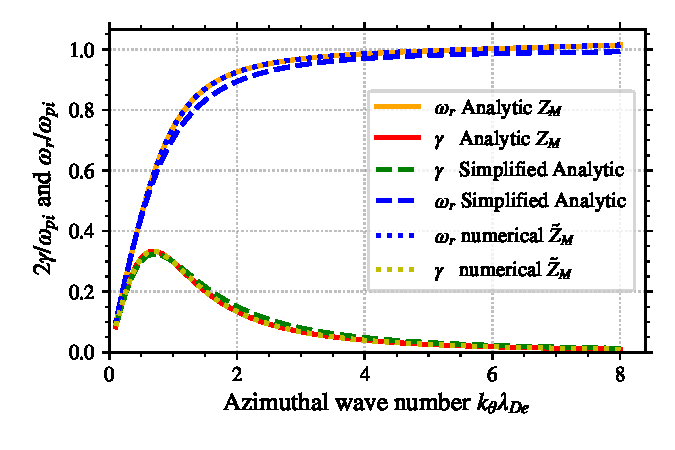
\includegraphics[width=\defaultwidth]{IAW_Maxw}
    \caption{\ac{IAW} frequency and growth rate for a Maxwellian distribution function using the Freid and Conte function (label Analytic $Z$), the numerical estimation of $\tilde{Z}$, and the simplified analytic expressions of \cref{eq-MIAW}. The wavevector is supposed in the azimuthal direction }
    \label{fig-IAW_Maxw}
  \end{figure}
  
  We can see that all results gives the same solution.
  The growth rates are all overlapping, hence it is difficult to see the differences.
  The simplified analytic expression returns a slightly different result, but the differences is negligible.
  The numerically evolution of $\tilde{Z}$ give the same result as analytic evaluation.
  
  \Cref{fig-IAW_druv} shows the effect of a Druyvesteyn electron distribution compared to a Maxwellian.
  We recall that a Druyvesteyn distribution follows the expression
  \begin{equation} \label{eq-druyv}
    f_{D}(v) = \exp \lp C1 \frac{\norm{v}^3}{v_{th}^3}  \rp C2,
  \end{equation}
  with $C1 \simeq 0.63$ and $C2 \sim 0.84$ two normalizing constants.
  We can see that there is no much impact of the Druyvesteyn electron velocity distribution function on the electron, except that the growth rate is sightly diminished.
  
  \begin{figure}[hbtp]
    \centering
    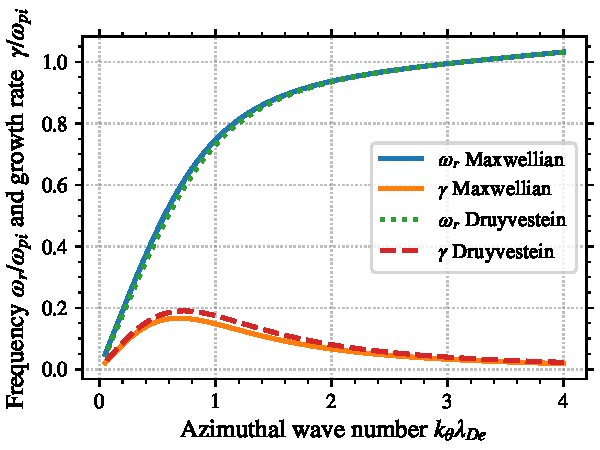
\includegraphics[width=\defaultwidth]{IAW_druv}
    \caption{\ac{IAW} frequency and growth rate for a Maxwellian distribution function using the Freid and Conte function and a Druyvesteyn distribution evaluated with the numerical estimation of $\tilde{Z}$. The wavevector is supposed in the azimuthal direction }
    \label{fig-IAW_druv}
  \end{figure}
  
  \paragraph{Electron Cyclotron Drift instability\\}
  
    \Cref{fig-ECDI_druv} shows the frequency and the grow rate for the \ac{ECDI}, using defined by \cref{eq-drECDI}, in the same conditions that the \ac{IAW} results, with $k_r \lambda_{De} = 0.1 $.
    The infinite sum over the cyclotron resonances is stopped at $N_{max} = 20$.
    
    
    \begin{figure}[hbtp]
    \centering
    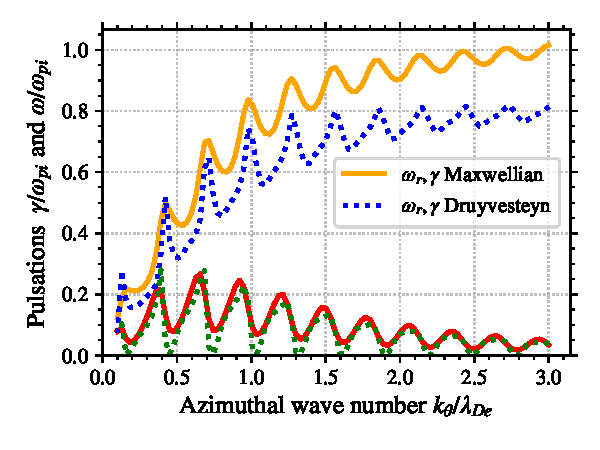
\includegraphics[width=\defaultwidth]{ECDI_druv}
    \caption{\ac{ECDI} frequency and growth rate for a Maxwellian distribution function using the Freid and Conte function and a Druyvesteyn distribution evaluated with the numerical estimation of $\tilde{Z}$, the radial wave number is $k_r \lambda_{De} = 0.1 $.}
    \label{fig-ECDI_druv}
  \end{figure}
  
  We can see in \cref{fig-ECDI_druv} that the cyclotron resonances are present for both distribution functions.
  But while the growth rate is not much affected, the frequency is reduced for larger azimuthal wave number.
  
  For a smaller radial wavenumber, the numerical resolution cashes as the argument in the $Z$ function diverges.
  However, in the limit $\eta \rightarrow \infty, Z(\eta) \rightarrow  \frac{1}{\eta}$.
  Hence, still obtain the cyclotron resonances, as shown in \citet{janhunen2018}, Fig. 2.

  \subsection{Distribution function measured} \label{subsec-VDFpic}
  
  Before solving the dispersion relation for the \ac{PIC} distribution function, let take a look to the distribution functions.
  
  \Cref{fig-vdfs_pic_time} shows at different moments in the simulation the ion and electron azimuthal velocity distribution functions, normalized.
  The velocities are normalized by the thermal speed of the species.
  To guide the reading of the figure, is added a Maxwellian distribution function as well as the electron theoretical drift velocity $u_e = \frac{E_z}{B_r}$, normalized to the electron thermal speed.
  The distributions are averages in time over $4\,\nano\second$, and in space over all the azimuthal direction.
  In the radial direction, the distributions are average over a small length at the center between the wall, between $r=0.45\,\centi\meter$ and $r=0.55\,\centi\meter$.
  
  \begin{figure}[hbtp]
    \centering
    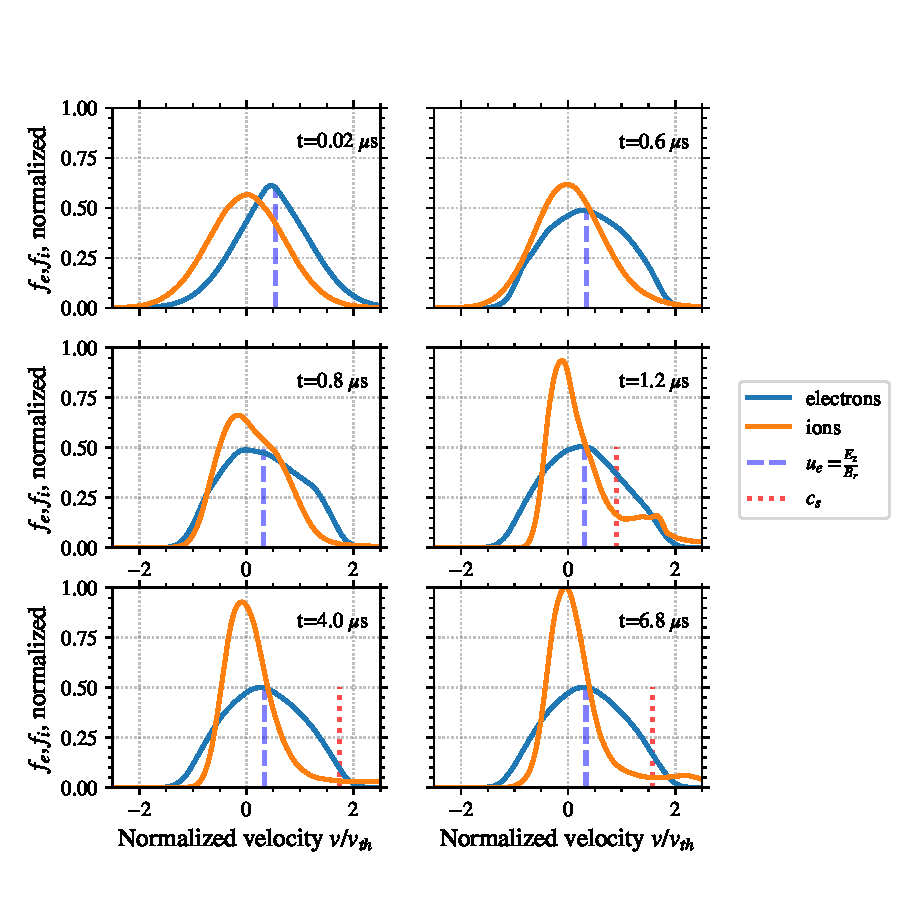
\includegraphics[width=0.8\textwidth]{Distributions_time_evolution_2.pdf}
    \caption{Electron and ion normalized azimuthal velocity distribution functions. The velocity in abscissa is normalized by the thermal speed of the corresponding species. Is overlaid a Maxwellian distribution, the theoretical $E\times B$ drift velocity of the electrons $u_e = \frac{E_z}{B_r}$, and the ion sound speed $c_s$ normalized by the ion velocity.}
    \label{fig-vdfs_pic_time}
  \end{figure}
  
  We can observe in \cref{fig-vdfs_pic_time} that the electron mean velocity is always the $E \times B$ drift velocity, which is is of the order of one quarter of the electron thermal speed.
  On the other hand, at the beginning of the simulation the mean velocity of the ion is null.
  But we can see that starting from $t=.8\,\micro\second$, the ions are dragged in the same direction that the electron drift.
  Here, we have to be careful not to misread the figure.
  As we have $v_{th, e} > v_{th, i}$, the effective drift velocity of the ion is much less that the electron.
  \inlinenote{Give the values here}
  \inlinenote{Maybe Do 2 figures ?  So that it is more readable ?}
  
  We can see a small population of high energy ions is generated.
  This leads to both an increases ion temperature, and the formation of a drift velocity in the azimuthal direction.
  The high energy ion population comes from ion trapping, as we can see that their velocity if of the order of the ion sound speed, which is close tot he wave phase velocity \citet{lafleur2018}.
  
  \vspace{1em}
  As both electron and ion velocity distribution functions are far from a drifting Maxwellian, we will use both of same in the calculations of the dispersion relation.
  
  
  
  \subsection{electron cyclotron drift instability} \label{subsec-VDFpic}
  
    \inlinenote{Ici: le debut, la partie linear. Montrer les resonances. Dire que la DR EVDI n'est plus utile après (fig ECDI_PIC_time.pdf)}
  
  
  
  
  \subsection{Ion acoustic wave} \label{subsec-VDFIAW}
  
  
  
  \begin{figure}[hbtp]
    \centering
    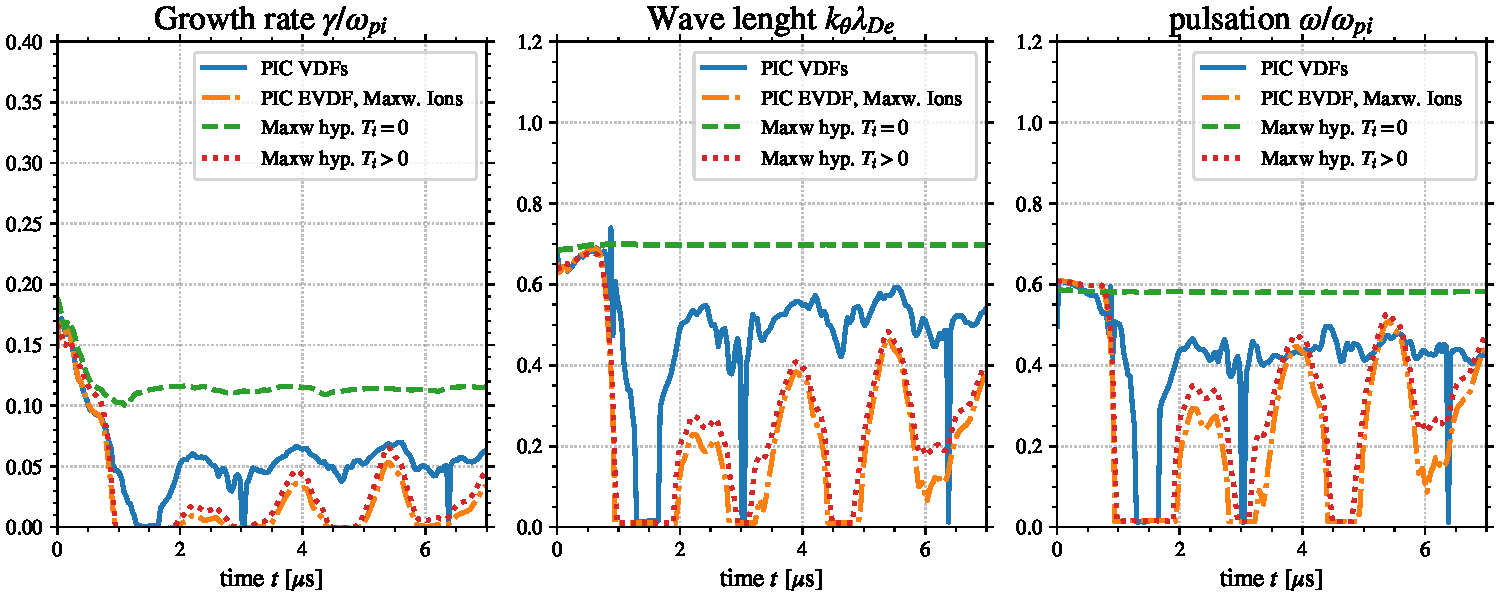
\includegraphics[width=0.8\textwidth]{GrowthRate_time_evolution_250_ter.pdf}
    \caption{Temporal evolution of the growth rate $\gamma$, the azimuthal wavenumber $k$ and the frequency $\omega$ for the most growing wave, obtained with several hypothesis on the dispersion relation. See text for more precisions. }
    \label{fig-time_wave}
  \end{figure}
  